\problemname{Hailstone Numbers}

\begin{minipage}[t]{0.5\textwidth}
\vspace{0pt}
Imagine writing down all positive integers on an infinitely large
piece of paper. From each number $n>1$ you now draw an arrow to the number
\begin{itemize}
\item $n/2$ \ \ \ \ \ \ if $n$ is even.
\item $3n+1$ \ if $n$ is odd.
\end{itemize}

An excerpt from the graph that is formed is shown in the comic panel next to this text. The
sequences you get by following the arrows are sometimes called \emph{hailstone numbers} because, like
hailstones, they drift up and down along the number line before finally falling
down to the ground (the number 1). The interesting thing is that it still has not been proven that
you always reach the number 1, but it has been
verified for all numbers up to $10^{19}$ so one \emph{conjectures} it, which is usually called the Collatz conjecture.

Write a program that, given two different integers, computes how far apart (number of arrows,
regardless of direction) they are in the graph.

\vfill
\end{minipage}
\begin{minipage}[t]{0.4\textwidth}
\vspace{0pt}
%\begin{figure}[!h]
\begin{center}
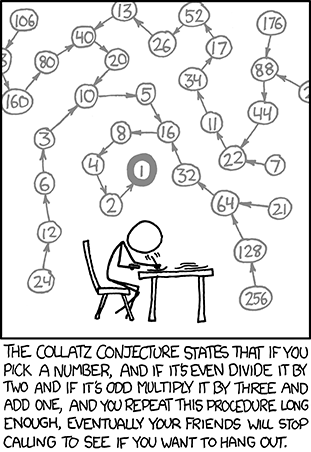
\includegraphics[width=0.8\textwidth]{collatz.png} \\
\tt{http://xkcd.com/710/}
\end{center}
%\end{figure}


\end{minipage}

\section*{Input}
The first and only line contains the integers $A$ and $B$ ($1\leq A,B \leq 1000$).

\section*{Output}
Output an integer: the number of steps between $A$ and $B$ in the graph.

\section*{Scoring}
Your solution will be tested on a set of test groups.
To earn points for a group, you must pass all test cases in that group.

\noindent
\begin{tabular}{| l | l | p{12cm} |}
  \hline
  \textbf{Group} & \textbf{Points} & \textbf{Constraints} \\ \hline
  $1$    & $40$       & $A=1$ \\ \hline
  $2$    & $60$       & No additional constraints. \\ \hline
\end{tabular}
